\documentclass[12pt,a4paper]{article}
\usepackage[utf8]{inputenc}
\usepackage{fancyhdr}
\usepackage{datetime2}
\usepackage{parskip}
\usepackage{lipsum}
\usepackage{graphicx}
\usepackage{float}

\pagestyle{fancy}
\fancyhf{}

\lhead{eriro331, micso554}
\rhead{\today} % yyyy-mm-dd
\setlength{\headheight}{15pt}

\cfoot{\thepage}

\begin{document}

\begin{center}
	\Huge
	\textbf{TDDC17 - AI}

	\vspace{0.3cm}
	\Large
	Erik Rönmark
	Michael Sörsäter
	
	\vspace{0.7cm}
	\textbf{Lab2 report}
\end{center}

\textbf{1. In the vacuum cleaner domain in part 1, what were the states and actions? What is the branching factor?}

Initial state, where the agent starts. Goal state, when the agent is done. All states between are called the problem states. The actions are: move up, down, left, right and suck dirt.

The branching factor is 4.


\textbf{2. What is the difference between Breadth First Search and Uniform Cost Search in a domain where the cost of each action is 1?}

There is no difference. If actions cost can vary, then Uniform Cost Search is better.


\textbf{3. Suppose that h1 and h2 are admissible heuristics (used in for example A*). Which of the following are also admissible?
a) (h1+h2)/2
b) 2h1
c) max (h1,h2)}

Both A and C are admissible. A because h1 and h2 are both admissible and the average of them can't be greater than either h1 or h2. C because even if h2 is greater than h1, it's still admissible. 

\textbf{4. If one would use A* to search for a path to one specific square in the vacuum domain, what could the heuristic (h) be? The cost function (g)? Is it an admissible heuristic?}

H(n): An example could be the shortest straight path if ignoring obstacles from the current node to the goal node.

G(n): The cost from the initial node to the current node.

Yes, it's an admissible heuristic.

\newpage

\textbf{5. Draw and explain. Choose your three favorite search algorithms and apply them to any problem domain (it might be a good idea to use a domain where you can identify a good heuristic function). Draw the search tree for them, and explain how they proceed in the searching. Also include the memory usage. You can attach a hand-made drawing.}

\begin{figure}[ht]
	\centering
	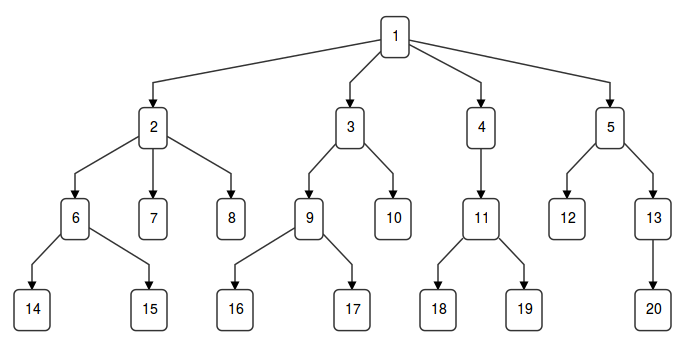
\includegraphics[width=0.6\textwidth]{graph}
	\caption{The tree used in all examples}
\end{figure}

All algorithms terminates when reaching the goal (F).

The order for Breadth First Search: \\
A, B, C, D, E, F \\
Memory usage: $\mathcal{O}(b^d)$

The order for Depth Fist Search: \\
A, B, D, E, H, F \\
Memory usage: $\mathcal{O}(bm)$

The order for Uniform Cost Search: \\
A, C, B, G, E, F \\
Memory usage: $\mathcal{O}(b^{1+\lfloor\frac{C^*}{\epsilon}\rfloor})$

b = branching factor, d = depth of the shallowest solution, m = maximum depth of the tree, C* = optimal solution, $\epsilon$ = positive integer

\textbf{6. Look at all the offline search algorithms presented in chapter 3 plus A* search. Are they complete? Are they optimal? Explain why!}

Breadth First is complete since it is guaranteed to find the goal if it exists, it is also optimal for unit step costs, otherwise it will return the shortest path (in steps) but not neccesary in cost.

Uniform Cost algorithm is complete as long as the branching factor is finite and all costs are positive. It is optimal.

Depth First is not complete when applied to infinite graphs, since it can get lost in a part without a goalstate. Otherwise it is complete. It is however not optimal, as it may ignore cheaper paths if it reaches the goal early.

Depth Limited is not complete and not optimal. It is similar to Depth First but have a specified search limit which means it can find a solution in a finite search space where Depth First will fail. 

Iterative Deepening is similar to Breadth First but uses less memory. On each iteration it uses Depth First to explore nodes. It is both optimal and complete.

Bidirectional searches in two directions in the search space. It is optimal if all costs are equal and if both directions use Breadth First. It is complete if the branching factor is finite and if both directions use Breadth First.

A* is optimal like Breadth First and complete because it will always find a solution.


\textbf{7. Assume that you had to go back and do Lab 1/Task 2 once more (if you did not use search already). Remember that the agent did not have perfect knowledge of the environment but had to explore it incrementally. Which of the search algorithms you have learned would be most suited in this situation to guide the agent's execution? What would you search for? Give an example.}

We chose to use Breadth First Search. It's a good algorithm because it quickly finds an unknown node. To use A* would be better because BFS doesn't take into account that rotation have a cost.

\end{document}